
\begin{figure}[t!]
    \centering
    \captionsetup{type=figure}
    \begin{subfigure}[t]{0.48\linewidth}
        \centering
        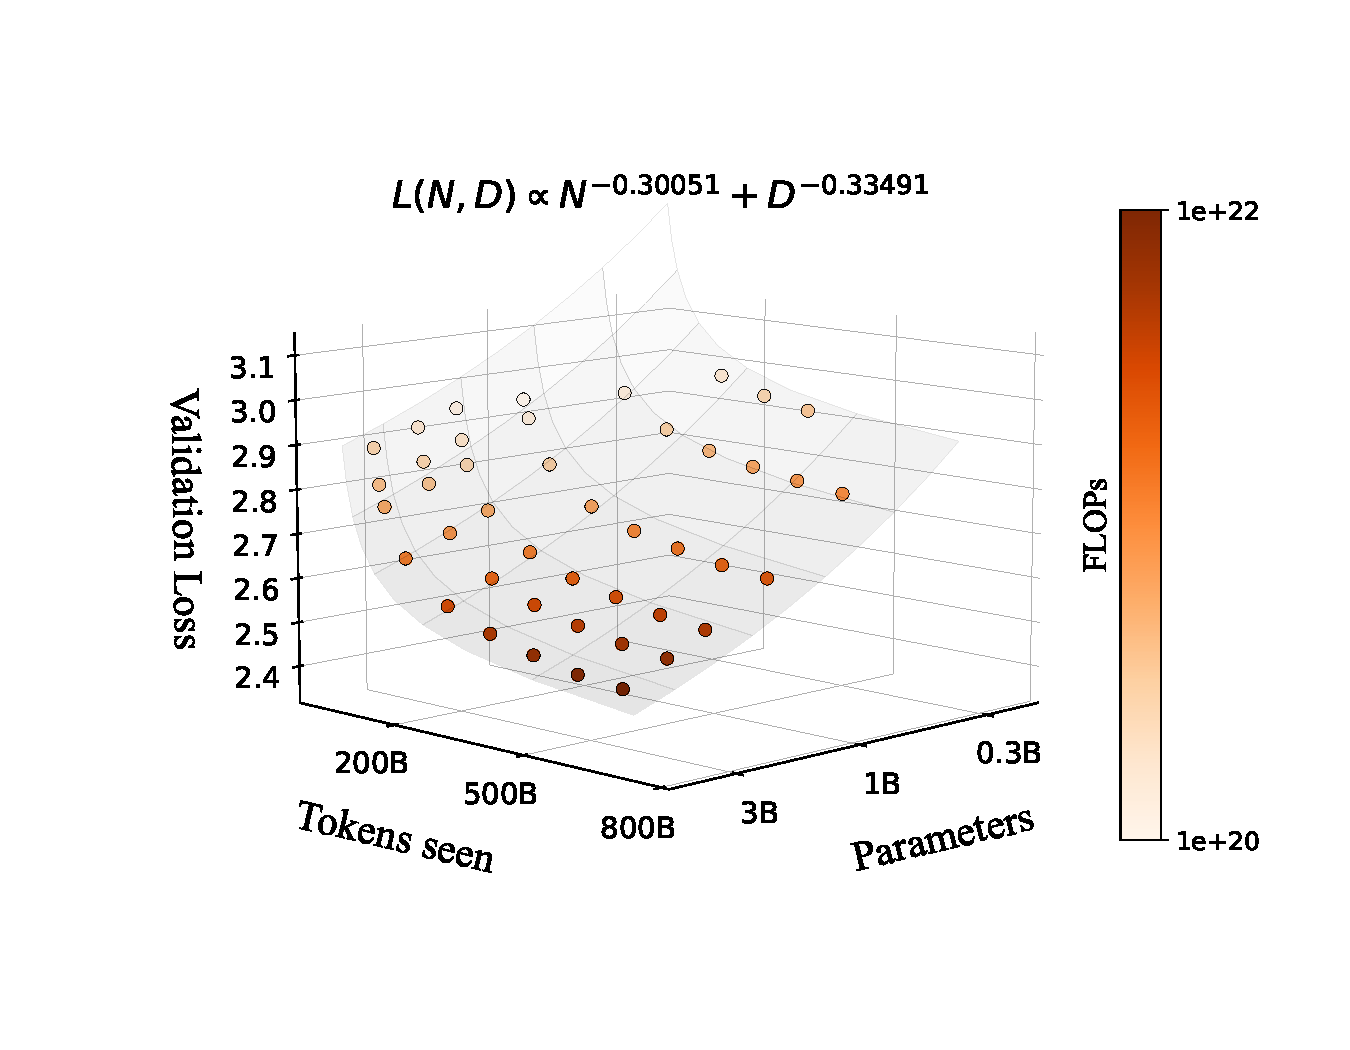
\includegraphics[width=1.02\linewidth]{assets/early/3d_scaling_early.pdf}
    \end{subfigure}
    \hfil
    \begin{subfigure}[t]{0.48\linewidth}
        \centering
        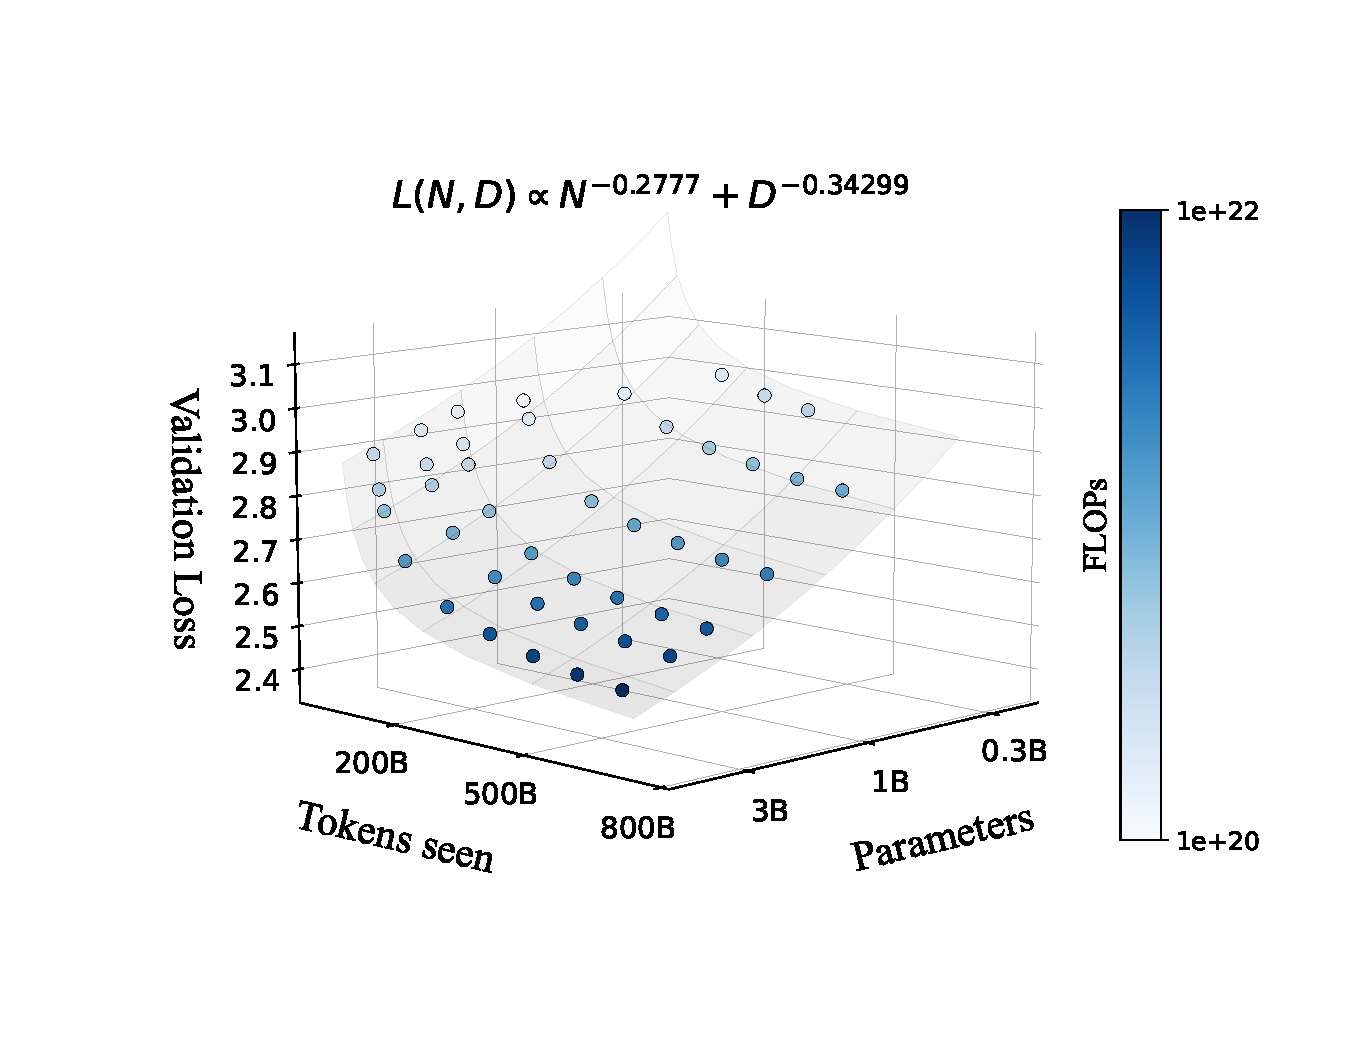
\includegraphics[width=1.02\linewidth]{assets/early/3d_scaling_late.pdf}
    \end{subfigure}
    \vspace{5pt}
    \setlength{\fboxsep}{0.5pt}
    \setlength{\fboxrule}{0pt}
    \caption{\textbf{适用于\fbox{\colorbox{CustomC_Light1!20}{\strut
    提前融合}}和\fbox{\colorbox{CustomD_Light1!20}{延迟融合\strut}}
    原生多模态模型的缩放规律。} 每个点代表一个模型(300M到3B参数),在不同数量的词元(250M到400B)上进行训练。我们在\edit{交错数据(Obelics)、图像-标题数据(HQITP)以及仅文本数据(DCLM)}的有效验证集上报告平均交叉熵损失。}
    \label{fig:early_vs_late_scaleflops_3d}
\end{figure}
